% Fig. 1: study architecture diagram (double column), ISPRS JPRS paper.
% Build:  pdflatex -interaction=nonstopmode fig01_workflow_tikz.tex
%         (driven by src/figures/build_fig01.py, which also writes the 600 dpi PNG)
% Output: figures/fig01_workflow.pdf  (natural width exactly 522.0 TeX pt = DOUBLE_COL,
%         so \includegraphics[width=\textwidth] in the final 5p layout scales by 1.0 and
%         the font sizes set below are the printed sizes).
%
% Numbers drawn in the diagram come from tables/data_summary.csv (one key per number):
%   7,572  -> key txt.all.n_rows        (all rows of data/processed/gloria.parquet)
%   6,957  -> key txt.all.n_qc_primary  (rows with qc_primary)
%   387    -> key txt.all.n_wb_group    (distinct wb_group over all rows)
% No result value appears in this figure.
%
% Content follows research/PREREGISTRATION.md sections 1-3 with Amendments 1-5
% (contributor unit = Dataset_ID folds, A1.2; region leave-one-out, A1.3; CV+ K = 10, A2.1,
% A4.1, A5.1; normalised split conformal, prereg 3) and research/EXPERIMENT_PLAN.md.
%
% Geometry (TeX pt, y downward). Picture 522.0 x 250.0 pt = 7.223 x 3.459 in.
%   stage strip  x   6 .. 58   (label text width 52)
%   content      x  70 .. 516  (446 pt)
%   panel 1  y    0 .. -85     4 boxes, w 100, gaps 15.33, x 70 / 185.33 / 300.67 / 416
%   panel 2  y  -99 .. -140    same 4 columns
%   panel 3  y -154 .. -250    boxes w 96 / 206 / 108, gaps 18, x 70 / 184 / 408
\documentclass[border=0pt]{standalone}
\usepackage{iftex}
\ifPDFTeX                      % fallback path: pdflatex cannot embed the system Arial
\usepackage[T1]{fontenc}
\usepackage{helvet}            % URW Nimbus Sans: Helvetica metrics. The Elsevier artwork
\renewcommand{\familydefault}{\sfdefault}  % guide allows "Arial (or Helvetica)".
\else                          % lualatex/xelatex: embed the same Arial as the matplotlib figures
\usepackage{fontspec}
% Name the faces explicitly: fontspec otherwise resolves Arial's italic to Arial Narrow Italic.
\setmainfont{Arial}[BoldFont=Arial Bold, ItalicFont=Arial Italic, BoldItalicFont=Arial Bold Italic]
\setsansfont{Arial}[BoldFont=Arial Bold, ItalicFont=Arial Italic, BoldItalicFont=Arial Bold Italic]
\renewcommand{\familydefault}{\sfdefault}
\fi
\usepackage{xcolor}
\usepackage{tikz}
\usetikzlibrary{positioning,arrows.meta,fit,backgrounds,calc}

% ---- Okabe-Ito palette (src/figures/style.py OKABE_ITO) -------------------------------
\definecolor{oiBlue}{HTML}{0072B2}
\definecolor{oiGreen}{HTML}{009E73}
\definecolor{oiVerm}{HTML}{D55E00}
\definecolor{oiPurple}{HTML}{CC79A7}
\definecolor{oiOrange}{HTML}{E69F00}
\definecolor{oiSky}{HTML}{56B4E9}
\definecolor{ink}{HTML}{1A1A1A}

% ---- type ----------------------------------------------------------------------------
\newcommand{\hdfont}{\fontsize{9}{11}\selectfont\bfseries}
\newcommand{\bdfont}{\fontsize{8}{11}\selectfont}
% box content: #1 = inner text width, #2 = inner height, #3 = heading, #4 = body lines
\newcommand{\boxtext}[4]{%
  \begin{minipage}[t][#2][t]{#1}\raggedright
    {\hdfont #3\par}\vspace{3pt}{\bdfont #4\par}%
  \end{minipage}}
% two sub-columns used by the interval-methods box
\newcommand{\twocolbody}[4]{%
  \begin{minipage}[t][66pt][t]{88pt}\raggedright
    {\bdfont\itshape #1\par}{\bdfont #2\par}%
  \end{minipage}\hspace{16pt}%
  \begin{minipage}[t][66pt][t]{94pt}\raggedright
    {\bdfont\itshape #3\par}{\bdfont #4\par}%
  \end{minipage}}
% stage strip label
\newcommand{\stagelab}[1]{\begin{minipage}[c]{52pt}\raggedright
    \fontsize{9}{11}\selectfont\bfseries #1\par\end{minipage}}

\begin{document}
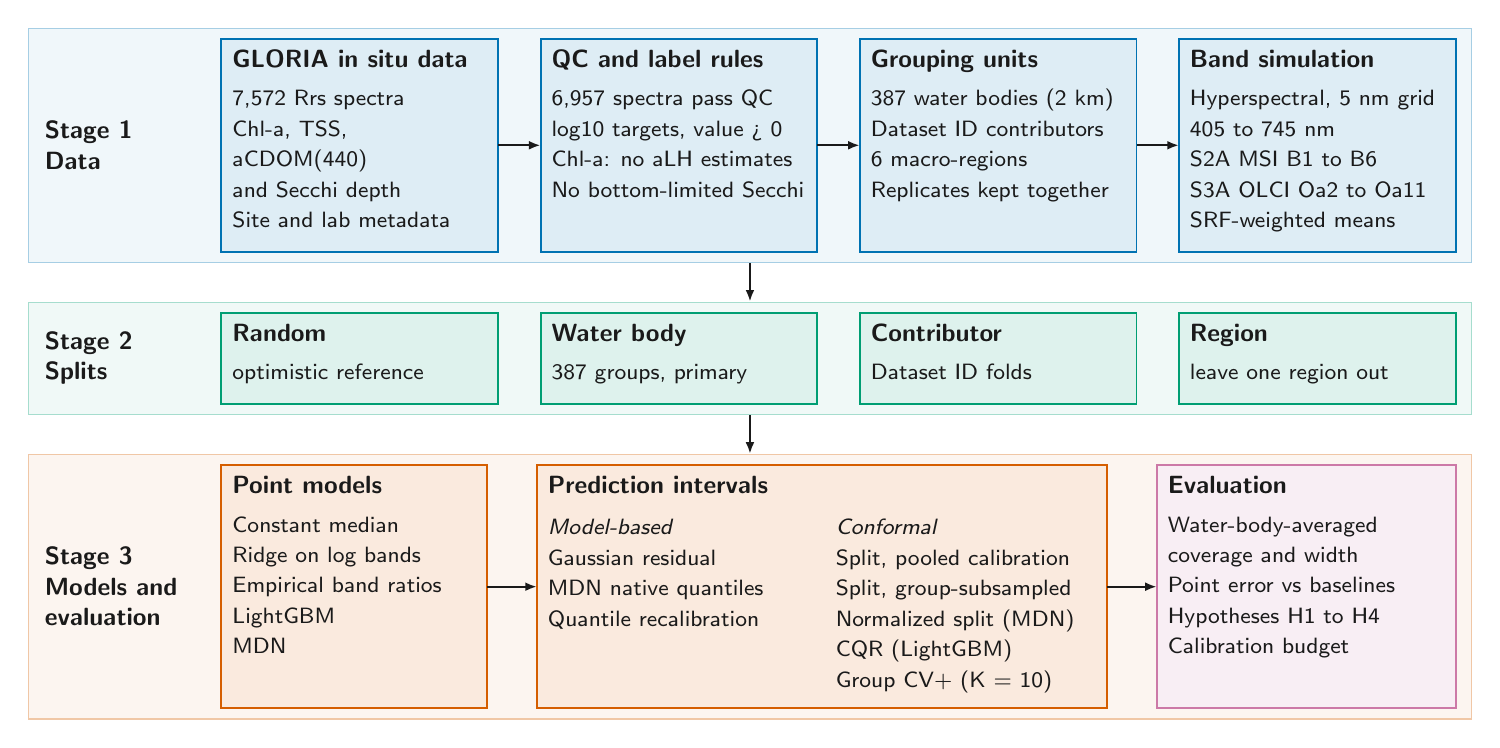
\begin{tikzpicture}[x=1pt,y=1pt,
    nbox/.style={draw=#1,line width=0.7pt,fill=#1!13!white,shape=rectangle,inner sep=4pt,
                 outer sep=0pt,anchor=north west,text=ink},
    flow/.style={-{Latex[length=4.2pt,width=3.2pt]},line width=0.8pt,draw=ink},
    stage/.style={anchor=west,text=ink,inner sep=0pt}]

\useasboundingbox (0,0) rectangle (522,-250);

% ======================= background panels (containers) ===============================
\fill[oiBlue!6!white]  (0,0)    rectangle (522,-85);
\fill[oiGreen!6!white] (0,-99)  rectangle (522,-140);
\fill[oiVerm!6!white]  (0,-154) rectangle (522,-250);
\draw[draw=oiBlue!35!white,line width=0.5pt]  (0.25,-0.25)   rectangle (521.75,-84.75);
\draw[draw=oiGreen!35!white,line width=0.5pt] (0.25,-99.25)  rectangle (521.75,-139.75);
\draw[draw=oiVerm!35!white,line width=0.5pt]  (0.25,-154.25) rectangle (521.75,-249.75);

% ======================= stage labels =================================================
\node[stage] at (6,-42.5)  {\stagelab{Stage 1\\Data}};
\node[stage] at (6,-119.5) {\stagelab{Stage 2\\Splits}};
\node[stage] at (6,-202)   {\stagelab{Stage 3\\Models and\\evaluation}};

% ======================= stage 1: data, units, sensor bands ===========================
\node[nbox=oiBlue] (d1) at (70,-4) {\boxtext{92pt}{69pt}{GLORIA in situ data}{%
7,572 Rrs spectra\\%
Chl-a, TSS, aCDOM(440)\\%
and Secchi depth\\%
Site and lab metadata}};
\node[nbox=oiBlue] (d2) at (185.33,-4) {\boxtext{92pt}{69pt}{QC and label rules}{%
6,957 spectra pass QC\\%
log10 targets, value > 0\\%
Chl-a: no aLH estimates\\%
No bottom-limited Secchi}};
\node[nbox=oiBlue] (d3) at (300.67,-4) {\boxtext{92pt}{69pt}{Grouping units}{%
387 water bodies (2 km)\\%
Dataset ID contributors\\%
6 macro-regions\\%
Replicates kept together}};
\node[nbox=oiBlue] (d4) at (416,-4) {\boxtext{92pt}{69pt}{Band simulation}{%
Hyperspectral, 5 nm grid\\%
405 to 745 nm\\%
S2A MSI B1 to B6\\%
S3A OLCI Oa2 to Oa11\\%
SRF-weighted means}};
\draw[flow] (170,-42.5)    -- (185.33,-42.5);
\draw[flow] (285.33,-42.5) -- (300.67,-42.5);
\draw[flow] (400.67,-42.5) -- (416,-42.5);

% ======================= stage 2: grouped splits ======================================
\node[nbox=oiGreen] (s1) at (70,-103)     {\boxtext{92pt}{25pt}{Random}{optimistic reference}};
\node[nbox=oiGreen] (s2) at (185.33,-103) {\boxtext{92pt}{25pt}{Water body}{387 groups, primary}};
\node[nbox=oiGreen] (s3) at (300.67,-103) {\boxtext{92pt}{25pt}{Contributor}{Dataset ID folds}};
\node[nbox=oiGreen] (s4) at (416,-103)    {\boxtext{92pt}{25pt}{Region}{leave one region out}};

% ======================= stage 3: models, intervals, evaluation =======================
\node[nbox=oiVerm] (m1) at (70,-158) {\boxtext{88pt}{80pt}{Point models}{%
Constant median\\%
Ridge on log bands\\%
Empirical band ratios\\%
LightGBM\\%
MDN}};
\node[nbox=oiVerm] (m2) at (184,-158) {\begin{minipage}[t][80pt][t]{198pt}\raggedright
    {\hdfont Prediction intervals\par}\vspace{3pt}%
    \twocolbody{Model-based}{%
Gaussian residual\\%
MDN native quantiles\\%
Quantile recalibration}{Conformal}{%
Split, pooled calibration\\%
Split, group-subsampled\\%
Normalized split (MDN)\\%
CQR (LightGBM)\\%
Group CV+ (K = 10)}%
  \end{minipage}};
\node[nbox=oiPurple] (m3) at (408,-158) {\boxtext{100pt}{80pt}{Evaluation}{%
Water-body-averaged\\%
coverage and width\\%
Point error vs baselines\\%
Hypotheses H1 to H4\\%
Calibration budget}};
\draw[flow] (166,-202) -- (184,-202);
\draw[flow] (390,-202) -- (408,-202);

% ======================= stage-to-stage arrows ========================================
\draw[flow] (261,-85)  -- (261,-99);
\draw[flow] (261,-140) -- (261,-154);

\end{tikzpicture}
\end{document}
